% Source: physical PDF pp. 91--95 (printed pp. 68--72). Coverage: Section 16.2 heading through the fermionic-determinant paragraph before Section 16.3; Eqs. (16.2.1)--(16.2.16), all intervening displays, Fig. 16.1, one citation, and one footnote. Uncertainty: none; the source's unsquared \mu(\phi_0) in Eq. (16.2.11) is preserved.
\subsection{Calculation of the Effective Potential}
\label{sec:16.2}

To see how the formalism of the previous section works in practice,
consider a simple example, the renormalizable theory of a single real
scalar field $\phi(x)$, with action
\begin{equation}
 I[\phi] = -\int d^4x\left[\lambda+\frac{1}{2}\partial_\rho\phi\partial^\rho\phi
 +\frac{1}{2}m^2\phi^2+\frac{1}{24}g\phi^4\right] .
 \tag{16.2.1}
 \label{eq:16.2.1}
\end{equation}
(We are here including a `cosmological constant' $-\lambda$ in the Lagrangian
density, for reasons that will become apparent.) Suppose for simplicity
that we wish to calculate $\Gamma[\phi_0]$ for a position-independent field $\phi_0(x) =
\phi_0$. Then every term in $\Gamma[\phi_0]$ will contain a factor of the volume of
spacetime

% Source: physical PDF p. 92 (printed p. 69). Coverage: complete four-panel Figure 16.1 and caption. Uncertainty: none; vector geometry reconstructed from the rendered scan.
\begin{figure}[htbp]
 \centering
 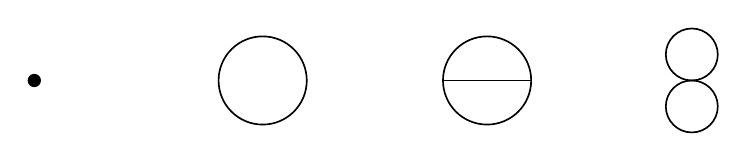
\begin{tikzpicture}[x=1cm,y=1cm,line width=0.6pt]
  % Zero loops: a point-like vacuum graph.
  \fill (0,0) circle[radius=2.4pt];

  % One loop.
  \draw (2.9,0) circle[radius=0.56];

  % Two loops: a circle divided by an internal chord.
  \draw (5.75,0) circle[radius=0.56];
  \draw (5.19,0) -- (6.31,0);

  % Two loops: a figure eight with the two loops meeting at one vertex.
 \draw (8.35,0.33) circle[radius=0.33];
 \draw (8.35,-0.33) circle[radius=0.33];
 \end{tikzpicture}
 \renewcommand{\thefigure}{16.1}
 \caption{Feynman diagrams with zero, one, or two loops for the quantum effective action of the theory of a neutral scalar field $\phi$ with interaction $\phi^4$.}
 \label{fig:16.1}
\end{figure}


\begin{equation}
 \mathcal{V}_4 = \int d^4x = \delta^4(p-p)(2\pi)^4
 \tag{16.2.2}
 \label{eq:16.2.2}
\end{equation}
arising from the momentum conservation delta-function. We will therefore
write, for $\phi_0$ constant
\begin{equation}
 \Gamma[\phi_0] = -\mathcal{V}_4 V(\phi_0) ,
 \tag{16.2.3}
 \label{eq:16.2.3}
\end{equation}
where $V(\phi_0)$ is an ordinary function, known as the \emph{effective potential}. In
this section we will calculate the effective potential to one-loop order.
This was originally done by Coleman and E.~Weinberg~\hyperref[ch16-ref-3]{[3]} in a study of
spontaneous symmetry breaking, the subject of Chapters 19 and 21. The
results were also used by them in one of the early applications of the
renormalization group, to be described in Section 18.2.

Shifting $\phi$ by $\phi_0$, the action in Eq.~\eqref{eq:16.1.18} is\footnote{There are limitations on the applicability of perturbation theory for $m^2<0$, discussed in the following section.}
\begin{align}
 I[\phi+\phi_0] ={}& -\mathcal{V}_4\left[\lambda+\frac{1}{2}m^2\phi_0^2+\frac{1}{24}g\phi_0^4\right]
 -\left[m^2\phi_0+\frac{1}{6}g\phi_0^3\right]\int d^4x\,\phi \notag\\
 &-\int d^4x\left[\frac{1}{2}\partial_\rho\phi\partial^\rho\phi
 +\frac{1}{2}\mu^2(\phi_0)\phi^2\right]
 -\int d^4x\left[\frac{1}{6}g\phi_0\phi^3+\frac{1}{24}g\phi^4\right] ,
 \tag{16.2.4}
 \label{eq:16.2.4}
\end{align}
where $\mu^2$ is the field-dependent mass
\begin{equation}
 \mu^2(\phi_0) = m^2+\frac{1}{2}g\phi_0^2 .
 \tag{16.2.5}
 \label{eq:16.2.5}
\end{equation}
Note that there now appear new interactions proportional to $\phi$ (which
have no effect on one-particle-irreducible graphs) and also $\phi^3$, as well as
terms with the same structure as those in the original action.

The Feynman diagrams for $\Gamma[\phi_0]$ with up to two loops are shown in
Figure~\ref{fig:16.1}. The zero-loop term in the vacuum--vacuum amplitude is just
given by the constant term in $I[\phi+\phi_0]$
\begin{equation}
 i\Gamma^{(0\ \mathrm{loop})}[\phi_0]
 = -i\mathcal{V}_4\left(\lambda+\frac{1}{2}m^2\phi_0^2+\frac{g}{24}\phi_0^4\right) .
 \tag{16.2.6}
 \label{eq:16.2.6}
\end{equation}

The one-loop term is given by
\begin{align}
 \exp\left(i\Gamma^{(1\ \mathrm{loop})}[\phi_0]\right)
 = \int\prod_x d\phi(x)\exp\Biggl\{&-\frac{1}{2}i\int d^4x
 \left[\partial_\rho\phi\partial^\rho\phi+\mu^2(\phi_0)\phi^2\right]
 \notag\\
 &{}+\epsilon\ \text{terms}\Biggr\} .
 \tag{16.2.7}
 \label{eq:16.2.7}
\end{align}
We learned how to calculate such integrals in Chapter 9; the result is
given by Eq.~(9.A.18):
\begin{equation}
 i\Gamma^{(1\ \mathrm{loop})}[\phi_0]
 = \ln\operatorname{Det}\left(\frac{iK}{\pi}\right)^{-1/2}
 = -\frac{1}{2}\operatorname{Tr}\ln\left(\frac{iK}{\pi}\right) ,
 \tag{16.2.8}
 \label{eq:16.2.8}
\end{equation}
where here
\begin{equation}
 K_{x,y} = \left[\frac{\partial^2}{\partial x^\lambda\partial y_\lambda}
 +\mu^2(\phi_0)-i\epsilon\right]\delta^4(x-y) .
 \tag{16.2.9}
 \label{eq:16.2.9}
\end{equation}
As usual, to calculate such traces it is helpful to diagonalize the `matrix'
$K$ by passing to momentum space:
\begin{align}
 K_{p,q} &= \int\frac{d^4x}{(2\pi)^2}e^{-ip\cdot x}
 \frac{d^4y}{(2\pi)^2}e^{iq\cdot y}K_{x,y} \notag\\
 &= \left(p^2+\mu^2(\phi_0)-i\epsilon\right)\delta^4(p-q) .
 \tag{16.2.10}
 \label{eq:16.2.10}
\end{align}
The logarithm of this diagonal matrix is just the diagonal matrix with
logarithms along the main diagonal:
% SOURCE NOTE: The scan visibly has \mu(\phi_0), without a superscript 2, in this equation.
\begin{equation}
 \left[\ln\left(\frac{iK}{\pi}\right)\right]_{p,q}
 = \ln\left[\frac{i}{\pi}\left(p^2+\mu(\phi_0)-i\epsilon\right)\right]\delta^4(p-q)
 \tag{16.2.11}
 \label{eq:16.2.11}
\end{equation}
and its trace is then
\begin{align}
 i\Gamma^{(1\ \mathrm{loop})}[\phi_0]
 &= -\frac{1}{2}\int d^4p\left[\ln\left(\frac{iK}{\pi}\right)\right]_{p,p} \notag\\
 &= -\frac{\mathcal{V}_4}{2(2\pi)^4}\int d^4p\,
 \ln\left(\frac{i}{\pi}\left(p^2+\mu^2(\phi_0)-i\epsilon\right)\right) .
 \tag{16.2.12}
 \label{eq:16.2.12}
\end{align}
Putting together Eqs.~\eqref{eq:16.2.6} and \eqref{eq:16.2.12}, we have the effective potential
to one-loop order
\begin{equation}
 V(\phi_0) = \lambda+\frac{1}{2}m^2\phi_0^2+\frac{g}{24}\phi_0^4
 +\mathcal{I}\bigl(\mu^2(\phi_0)\bigr) ,
 \tag{16.2.13}
 \label{eq:16.2.13}
\end{equation}
where
\begin{equation}
 \mathcal{I}(\mu^2) \equiv -\frac{i}{2(2\pi)^4}\int d^4p\,
 \ln\left(\frac{i}{\pi}\left[p^2+\mu^2-i\epsilon\right]\right) .
 \tag{16.2.14}
 \label{eq:16.2.14}
\end{equation}

It is painfully obvious that this formula for the effective potential
contains ultraviolet divergences. Fortunately, these are naturally absorbed
into a renormalization of the parameters of the theory. Although the
integral \eqref{eq:16.2.14} is divergent, simple power-counting shows that it is
made convergent by differentiating three times with respect to $\mu^2$:
\[
 \mathcal{I}'''(\mu^2) = -\frac{i}{(2\pi)^4}\int d^4p\,
 \left(p^2+\mu^2-i\epsilon\right)^{-3} .
\]
Once again, the $-i\epsilon$ term tells us that we must rotate the $p^0$ contour
counterclockwise, so that $p^0=ip_4$, with $p_4$ running from $-\infty$ to $+\infty$:
\[
 \mathcal{I}'''(\mu^2) = \frac{1}{(2\pi)^4}\int_0^\infty
 \frac{2\pi^2 k^3\,dk}{(k^2+\mu^2)^3} = \frac{1}{32\pi^2\mu^2} .
\]
Integrating thrice, we have then
\[
 \mathcal{I}(\mu^2) = \frac{\mu^4\ln\mu^2}{64\pi^2}+A+B\mu^2+C\mu^4 .
\]
The constants $A$, $B$, $C$ are not determined by this method of calculation,
which is hardly a serious problem since they are obviously infinite anyway.
We eliminate these constants by defining `renormalized' values for $\lambda$, $m^2$,
and $g$:
\begin{align*}
 \lambda_R &\equiv \lambda+A+Bm^2+Cm^4 ,\\
 m_R^2 &\equiv m^2+gB+2gm^2C ,\\
 g_R &\equiv g+6g^2C .
\end{align*}
Our final result for the potential to one-loop order is then
\begin{equation}
 V(\phi_0) = \lambda_R+\frac{1}{2}m_R^2\phi_0^2+\frac{g_R}{24}\phi_0^4
 +\frac{\mu^4(\phi_0)\ln\mu^2(\phi_0)}{64\pi^2} ,
 \tag{16.2.15}
 \label{eq:16.2.15}
\end{equation}
where $\mu(\phi_0)$ is the field-dependent mass defined by Eq.~\eqref{eq:16.2.5}, which to
this order can be calculated using $m_R$ and $g_R$ in place of $m$ and $g$:
\[
 \mu^2(\phi) = m_R^2+\frac{1}{2}g_R\phi^2 .
\]

Similar results hold if the theory contains a complex spin $\frac{1}{2}$ fermion
field $\psi(x)$ that interacts with the scalar $\phi$. For instance, if this interaction
Hamiltonian density has the simple form $G\phi\bar\psi\psi$, then the mass $M(\phi_0)$ of
the fermion in the presence of a constant scalar background field $\phi_0$ is of
the form:
\[
 M(\phi_0) = M(0)+G\phi_0 .
\]
It is easy to see that in this case the potential \eqref{eq:16.2.1} then receives an
additional term:
\begin{align}
 V(\phi_0) ={}& \lambda_R+\frac{1}{2}m_R^2\phi_0^2+\frac{g_R}{24}\phi_0^4
 +\frac{\mu^4(\phi_0)\ln\mu^2(\phi_0)}{64\pi^2} \notag\\
 &{}-\frac{M^4(\phi_0)\ln M^2(\phi_0)}{32\pi^2} .
 \tag{16.2.16}
 \label{eq:16.2.16}
\end{align}

The numerical coefficient in the new term is twice that of the $\mu^4\ln\mu^2$ term
in Eq.~\eqref{eq:16.2.15}, because of the two spin states of the fermion described by
$\psi$, while the sign is opposite because (as shown in Chapter 9) fermionic
path integrals of Gaussians give a result proportional to the determinant
of the matrix coefficient in the exponent, while bosonic path integrals of
Gaussians give a result proportional to the inverse of this determinant.
